\documentclass[12pt,a4paper]{scrartcl}
\usepackage[utf8]{inputenc}
\usepackage[english,russian]{babel}
\usepackage{indentfirst}
\usepackage{misccorr}
\usepackage{graphicx}
\usepackage{amsmath}
\graphicspath{}
\author{Даря}
\DeclareGraphicsExtensions{.pdf,.png,.jpg}
\begin{document}
\begin{flushright}
  Павлова Дарья\\
  19ПИ-1\\
  1.12.20\\
\end{flushright}

\textbf{Установка и настройка}
\\[5pt]
\textnumero 1. Samba
\\[5pt]
sudo apt install samba
\\[5pt]
+ соглашаемся на установку всех пакетов
\\[5pt]
Создаём резервную копию конфигурационного файла. Если что-то пойдет не так, то файл можно будет восстановить из копии
\\[5pt]
sudo cp /etc/samba/smb.conf /etc/samba/smb-b.conf
\\[5pt]
Создадим папку для шэринга и заполняем её чем-нибудь (у меня это файл cat1)
\\[5pt]
mkdir cats\_photos
\\[5pt]
Открываем конфигурационный файл 
\\[5pt]
sudo gedit /etc/samba/smb.conf 
\\[5pt]
-перейдем в конец файла и введем следующие строчки:
\\[5pt]
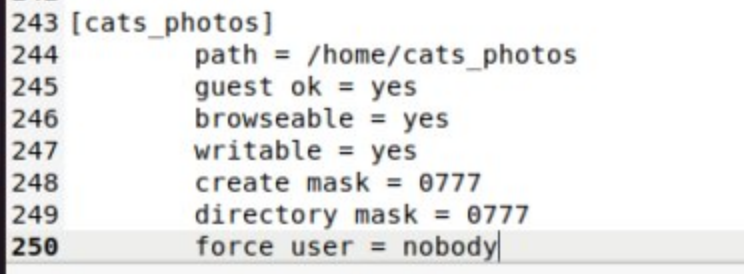
\includegraphics[scale=10, width=10cm]{f1}
\\[5pt]
Перезапускаем самбу
\\[5pt]
sudo service smbd restart
\\[5pt]
\textnumero 2. nginx
\\[5pt]
sudo apt install nginx
\\[5pt]
+ соглашаемся на установку всех пакетов
\\[5pt]
делаем бэкаб конфигов
\\[5pt]
sudo cp /etc/nginx/sites-available/default /etc/nginx/sites-available/default-b
\\[5pt]
sudo gedit /etc/nginx/sites-available/default
\\[5pt]
записываем в файлик данные строчки 
\\[5pt]
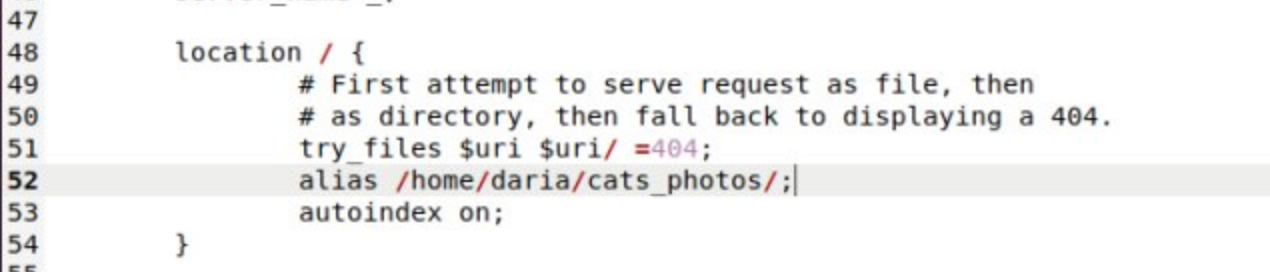
\includegraphics[scale=10, width=15cm]{f2}
\\[5pt]
\textbf{Настройка сети}
\\[5pt]
Настраиваем режим сетевого подключения в виртуальной машине
\\[5pt]
host-only означает, что наш ip будет доступен только на той машине, на котором запущена виртуальная машина
\\[5pt]
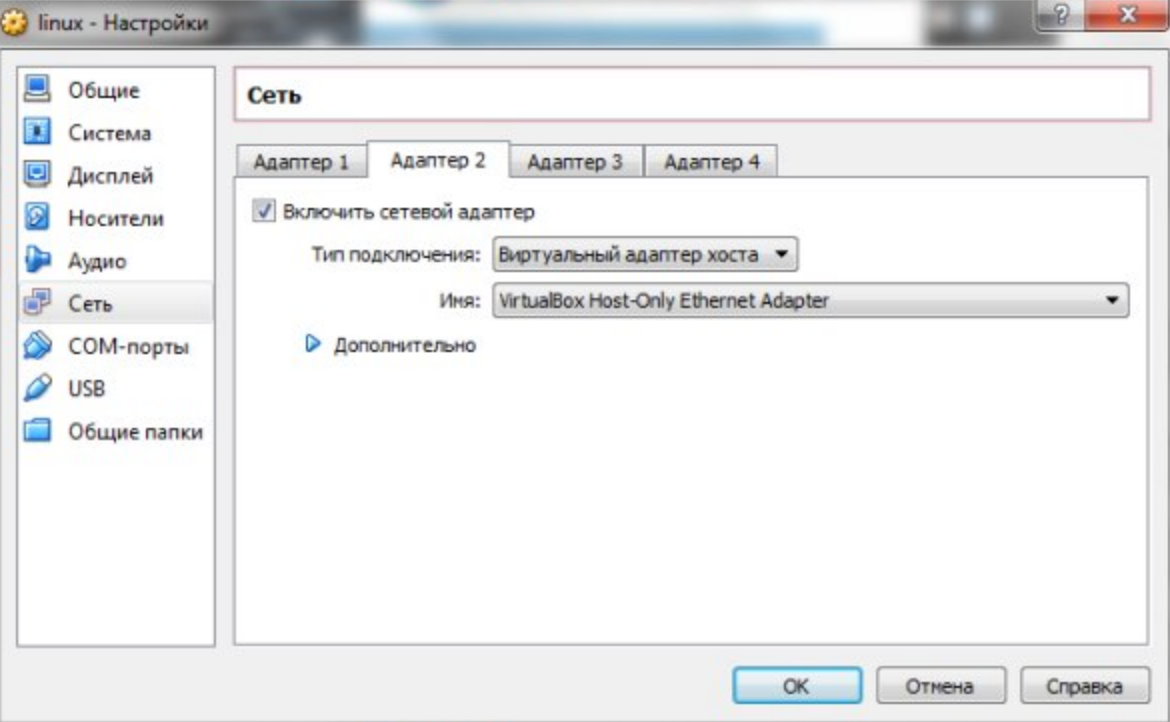
\includegraphics[scale=10, width=15cm]{f3}
\\[5pt]
узнаем ip
\\[5pt]
sudo apt install net-tools
\\[5pt]
sudo ifconfig
\\[5pt]
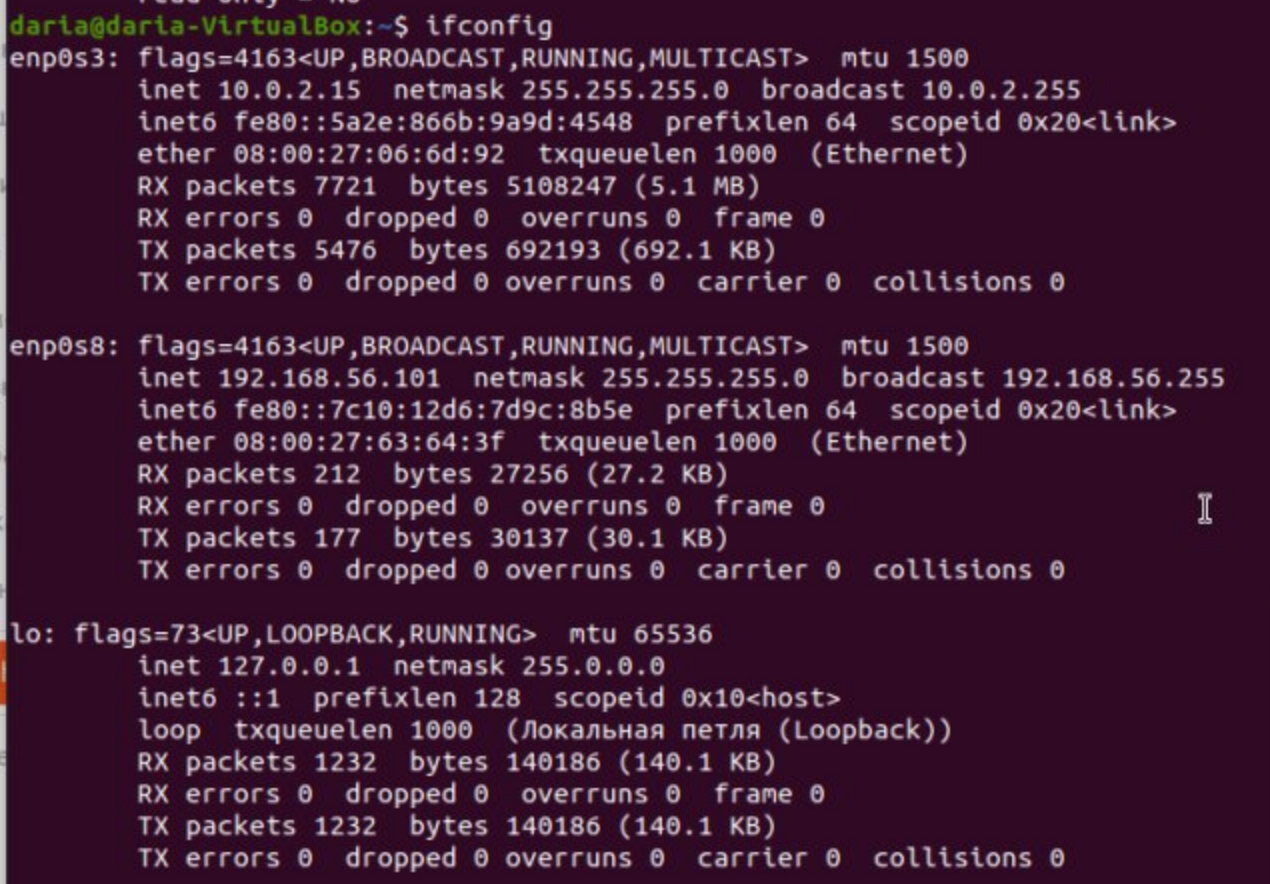
\includegraphics[scale=10, width=15cm]{f4}
\\[5pt]
10.0.2.15 - локальный ip для самбы
\\[5pt]
192.168.56.101 - хостовой ip заходим по нему через windows
\\[5pt]
\textbf{Просмотр расшаренной папки nginx}
\\[5pt]
\textnumero 1. через linux: \\[5pt]
http://localhost \\[5pt]
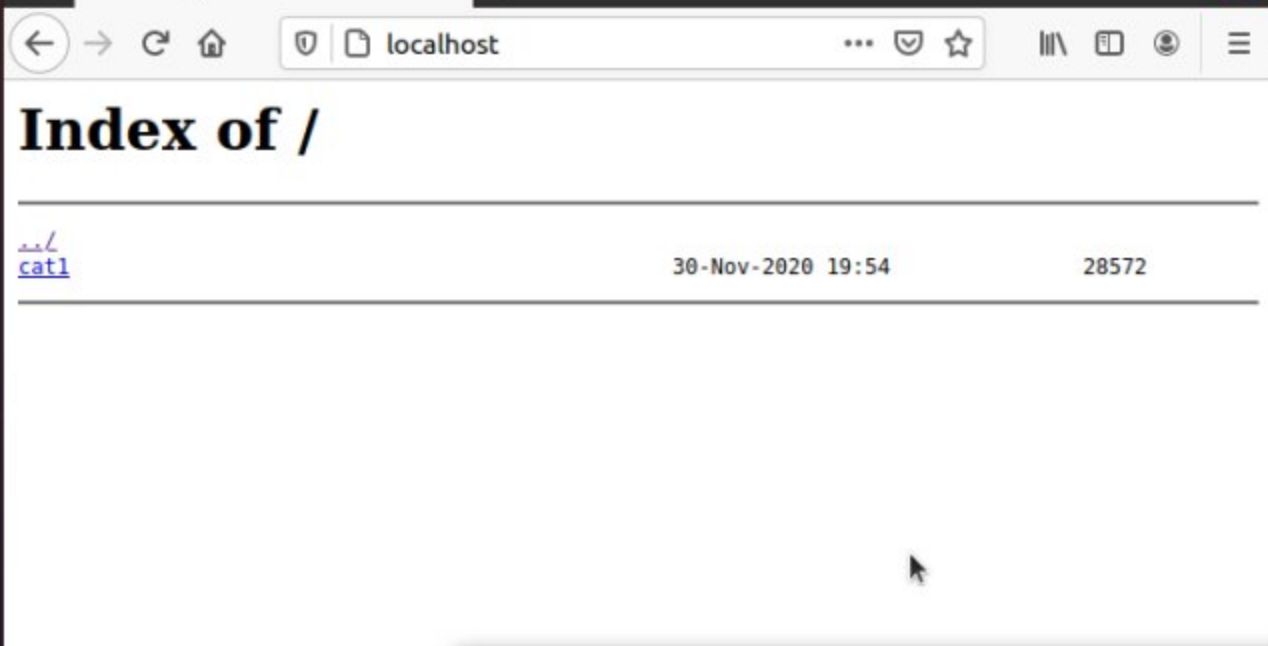
\includegraphics[scale=10, width=15cm]{f5}
\\[5pt]
\textnumero 2. через windows: \\[5pt] 
http://192.168.56.101 \\[5pt]
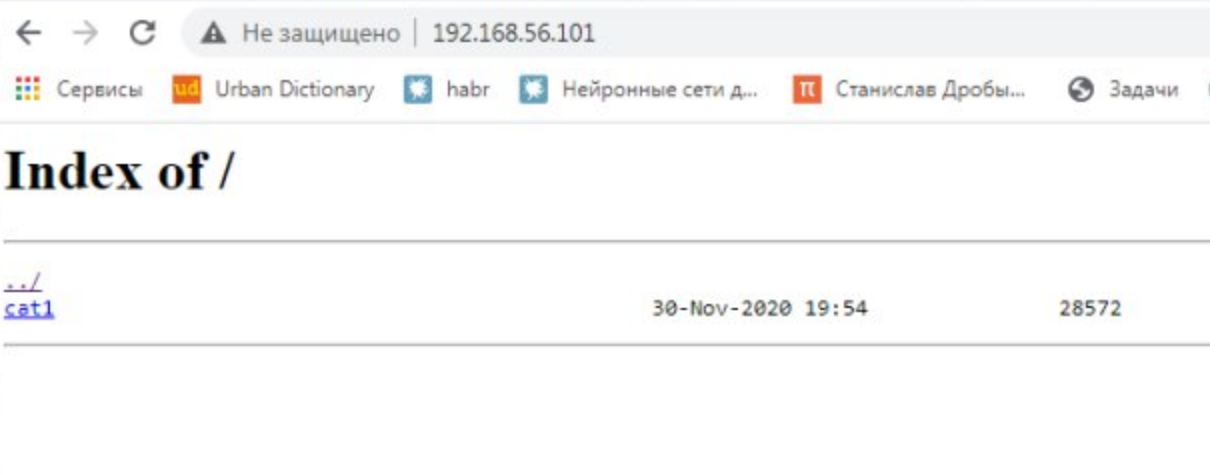
\includegraphics[scale=10, width=15cm]{f6} \\[5pt]
\textbf{Просмотр расшаренной папки samba} \\[5pt]
\textnumero 1. через файловый менеджер linux: \\[5pt]
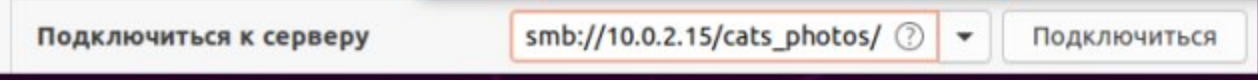
\includegraphics[scale=10, width=15cm]{f7} \\[5pt]
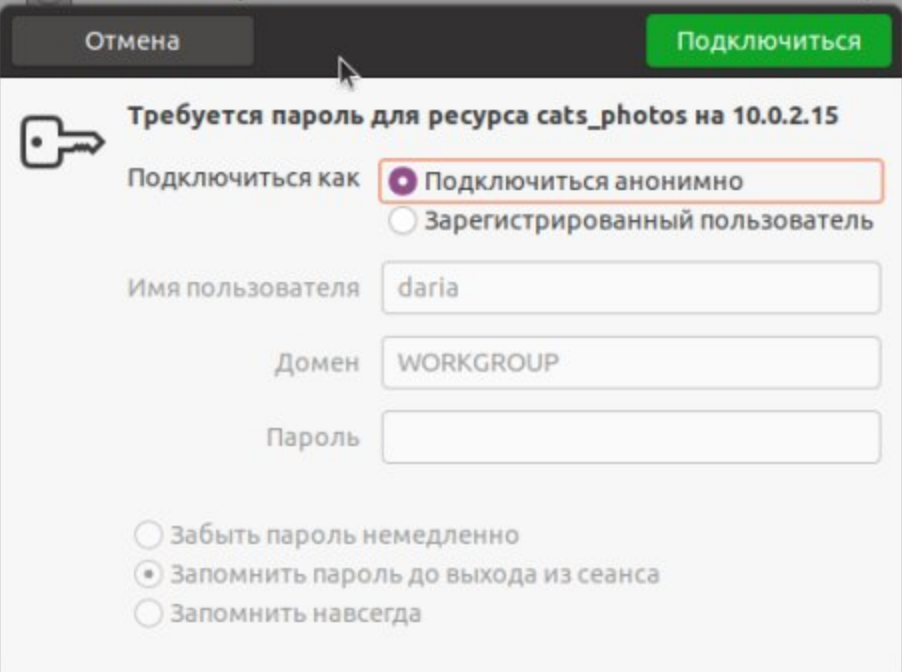
\includegraphics[scale=10, width=15cm]{f71} \\[5pt]
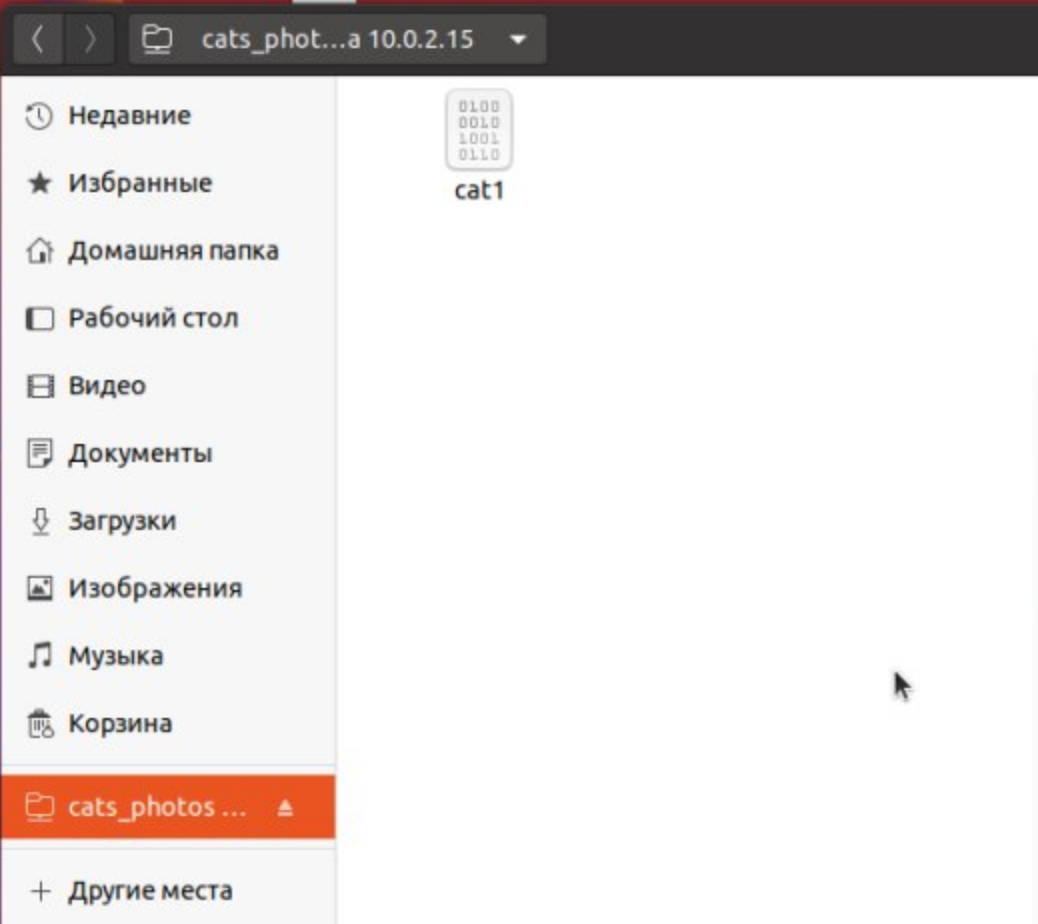
\includegraphics[scale=10, width=15cm]{f8} \\[5pt]
\textnumero 2. через файловый менеджер windows \\[5pt]
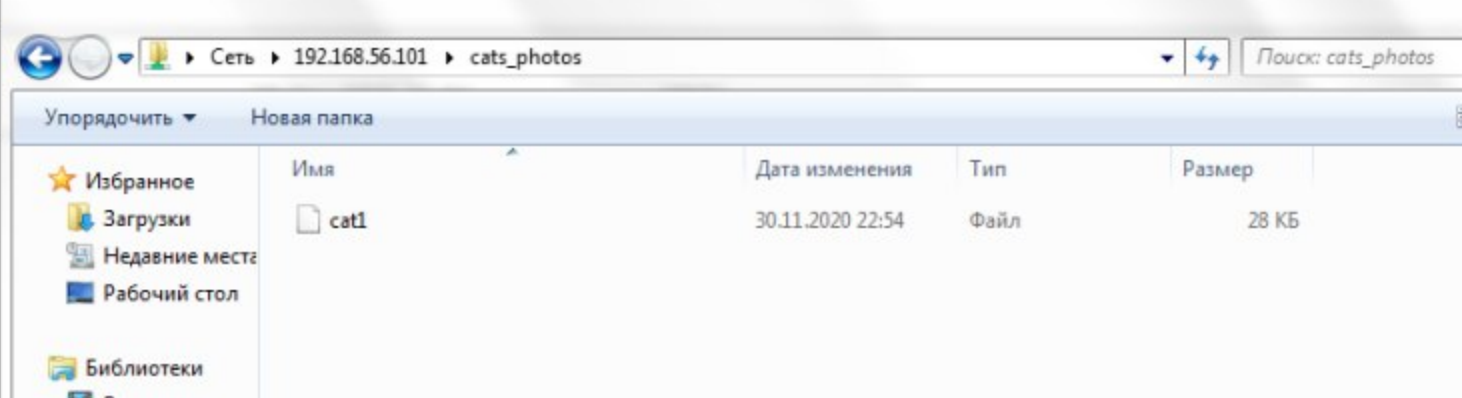
\includegraphics[scale=10, width=15cm]{f9}
\end{document}